%%%%%%%%%%%%%%%%%%%%%%%%%%%%%%%%%%%%%%%%%
%  My documentation report
%  Objetive: Explain what I did and how, so someone can continue with the investigation
%
% Important note:
% Chapter heading images should have a 2:1 width:height ratio,
% e.g. 920px width and 460px height.
%
%%%%%%%%%%%%%%%%%%%%%%%%%%%%%%%%%%%%%%%%%


%----------------------------------------------------------------------------------------
%	PACKAGES AND OTHER DOCUMENT CONFIGURATIONS
%----------------------------------------------------------------------------------------

\documentclass[6pt,oneside]{book} % Default font size and left-justified equations
\DeclareUnicodeCharacter{2212}{-}
\DeclareUnicodeCharacter{2217}{\odot}
\usepackage{hyperref}
\hypersetup{
    colorlinks=true,
    linkcolor=blue,
    filecolor=magenta,      
    urlcolor=cyan,
    pdftitle={Overleaf Example},
    pdfpagemode=FullScreen,
    }

\usepackage{amsmath}
\usepackage[utf8]{inputenc}

\usepackage{natbib} % Bibliography 
\setcitestyle{authoryear,open={(},close={)}}


\usepackage[top=3cm,bottom=3cm,left=3.2cm,right=3.2cm,headsep=10pt,letterpaper]{geometry} % Page margins

\usepackage{xcolor} % Required for specifying colors by name
\definecolor{ocre}{RGB}{52,177,201} % Define the orange color used for highlighting throughout the book

% Font Settings
\usepackage{avant} % Use the Avantgarde font for headings
%\usepackage{times} % Use the Times font for headings
\usepackage{mathptmx} % Use the Adobe Times Roman as the default text font together with math symbols from the Sym­bol, Chancery and Com­puter Modern fonts
\usepackage{microtype} % Slightly tweak font spacing for aesthetics
\usepackage[utf8]{inputenc} % Required for including letters with accents
\usepackage[T1]{fontenc} % Use 8-bit encoding that has 256 glyphs
\usepackage{amsthm}


\usepackage{datatool,environ,newfile}
\NewEnviron{sortEnvironment}[1]{{%
  \let\par\DTLpar% Cannot include \par in content, so replace \par with \DTLpar
  \addtostream{sortOutput}{"#1","\BODY"}% Write section content to output file
}}
\AtBeginDocument{%
  \newoutputstream{sortOutput}% New output file
  \openoutputfile{sortContent.csv}{sortOutput}% Open output file
}
\AtEndDocument{%
  \closeoutputstream{sortOutput}% Close output file
  \DTLloaddb[
      noheader,
      keys={Title,Content}]
    {sortedSections}{sortContent.csv}% Load stored content
  \dtlsort{Title}{sortedSections}{\dtlcompare}% Sort stored content
  \DTLforeach{sortedSections}{\Title=Title,\Content=Content}
    {\section{\Title} \Content}% Print all content
}


%----------------------------------------------------------------------------------------
%	VARIOUS REQUIRED PACKAGES
%----------------------------------------------------------------------------------------

\usepackage{titlesec} % Allows customization of titles

\usepackage{graphicx} % Required for including pictures
\graphicspath{{Pictures/}} % Specifies the directory where pictures are stored
% \graphicspath{{Plots/}}
\usepackage{lipsum} % Inserts dummy text

\usepackage{tikz} % Required for drawing custom shapes

\usepackage[english]{babel} % English language/hyphenation

\usepackage{enumitem} % Customize lists
\setlist{nolistsep} % Reduce spacing between bullet points and numbered lists

\usepackage{booktabs} % Required for nicer horizontal rules in tables

\usepackage{eso-pic} % Required for specifying an image background in the title page

%----------------------------------------------------------------------------------------
%	MAIN TABLE OF CONTENTS
%----------------------------------------------------------------------------------------

\usepackage{titletoc} % Required for manipulating the table of contents

\contentsmargin{0cm} % Removes the default margin
% Chapter text styling
\titlecontents{chapter}[1.25cm] % Indentation
{\addvspace{15pt}\large\sffamily\bfseries} % Spacing and font options for chapters
{\color{ocre!60}\contentslabel[\Large\thecontentslabel]{1.25cm}\color{ocre}} % Chapter number
{}  
{\color{ocre!60}\normalsize\sffamily\bfseries\;\titlerule*[.5pc]{.}\;\thecontentspage} % Page number
% Section text styling
\titlecontents{section}[1.25cm] % Indentation
{\addvspace{5pt}\sffamily\bfseries} % Spacing and font options for sections
{\contentslabel[\thecontentslabel]{1.25cm}} % Section number
{}
{\sffamily\hfill\color{black}\thecontentspage} % Page number
[]
% Subsection text styling
\titlecontents{subsection}[1.25cm] % Indentation
{\addvspace{1pt}\sffamily\small} % Spacing and font options for subsections
{\contentslabel[\thecontentslabel]{1.25cm}} % Subsection number
{}
{\sffamily\;\titlerule*[.5pc]{.}\;\thecontentspage} % Page number
[] 

%----------------------------------------------------------------------------------------
%	MINI TABLE OF CONTENTS IN CHAPTER HEADS
%----------------------------------------------------------------------------------------

% Section text styling
\titlecontents{lsection}[0em] % Indendating
{\footnotesize\sffamily} % Font settings
{}
{}
{}

% Subsection text styling
\titlecontents{lsubsection}[.5em] % Indentation
{\normalfont\footnotesize\sffamily} % Font settings
{}
{}
{}
 
%----------------------------------------------------------------------------------------
%	PAGE HEADERS
%----------------------------------------------------------------------------------------

\usepackage{fancyhdr} % Required for header and footer configuration

\pagestyle{fancy}
\renewcommand{\chaptermark}[1]{\markboth{\sffamily\normalsize\bfseries\chaptername\ \thechapter.\ #1}{}} % Chapter text font settings
\renewcommand{\sectionmark}[1]{\markright{\sffamily\normalsize\thesection\hspace{5pt}#1}{}} % Section text font settings
\fancyhf{} \fancyhead[LE,RO]{\sffamily\normalsize\thepage} % Font setting for the page number in the header
\fancyhead[LO]{\rightmark} % Print the nearest section name on the left side of odd pages
\fancyhead[RE]{\leftmark} % Print the current chapter name on the right side of even pages
\renewcommand{\headrulewidth}{0.5pt} % Width of the rule under the header
\addtolength{\headheight}{2.5pt} % Increase the spacing around the header slightly
\renewcommand{\footrulewidth}{0pt} % Removes the rule in the footer
\fancypagestyle{plain}{\fancyhead{}\renewcommand{\headrulewidth}{0pt}} % Style for when a plain pagestyle is specified

% Removes the header from odd empty pages at the end of chapters
\makeatletter
\renewcommand{\cleardoublepage}{
\clearpage\ifodd\c@page\else
\hbox{}
\vspace*{\fill}
\thispagestyle{empty}
\newpage
\fi}

%----------------------------------------------------------------------------------------
%	THEOREM STYLES
%----------------------------------------------------------------------------------------

\usepackage{amsmath,amsfonts,amssymb,amsthm} % For math equations, theorems, symbols, etc

\newcommand{\intoo}[2]{\mathopen{]}#1\,;#2\mathclose{[}}
\newcommand{\ud}{\mathop{\mathrm{{}d}}\mathopen{}}
\newcommand{\intff}[2]{\mathopen{[}#1\,;#2\mathclose{]}}
\newtheorem{notation}{Notation}[chapter]

%%%%%%%%%%%%%%%%%%%%%%%%%%%%%%%%%%%%%%%%%%%%%%%%%%%%%%%%%%%%%%%%%%%%%%%%%%%
%%%%%%%%%%%%%%%%%%%% dedicated to boxed/framed environements %%%%%%%%%%%%%%
%%%%%%%%%%%%%%%%%%%%%%%%%%%%%%%%%%%%%%%%%%%%%%%%%%%%%%%%%%%%%%%%%%%%%%%%%%%
\newtheoremstyle{ocrenumbox}% % Theorem style name
{0pt}% Space above
{0pt}% Space below
{\normalfont}% % Body font
{}% Indent amount
{\small\bf\sffamily\color{ocre}}% % Theorem head font
{\;}% Punctuation after theorem head
{0.25em}% Space after theorem head
{\small\sffamily\color{ocre}\thmname{#1}\nobreakspace\thmnumber{\@ifnotempty{#1}{}\@upn{#2}}% Theorem text (e.g. Theorem 2.1)
\thmnote{\nobreakspace\the\thm@notefont\sffamily\bfseries\color{black}---\nobreakspace#3.}} % Optional theorem note
\renewcommand{\qedsymbol}{$\blacksquare$}% Optional qed square

\newtheoremstyle{blacknumex}% Theorem style name
{5pt}% Space above
{5pt}% Space below
{\normalfont}% Body font
{} % Indent amount
{\small\bf\sffamily}% Theorem head font
{\;}% Punctuation after theorem head
{0.25em}% Space after theorem head
{\small\sffamily{\tiny\ensuremath{\blacksquare}}\nobreakspace\thmname{#1}\nobreakspace\thmnumber{\@ifnotempty{#1}{}\@upn{#2}}% Theorem text (e.g. Theorem 2.1)
\thmnote{\nobreakspace\the\thm@notefont\sffamily\bfseries---\nobreakspace#3.}}% Optional theorem note

\newtheoremstyle{blacknumbox} % Theorem style name
{0pt}% Space above
{0pt}% Space below
{\normalfont}% Body font
{}% Indent amount
{\small\bf\sffamily}% Theorem head font
{\;}% Punctuation after theorem head
{0.25em}% Space after theorem head
{\small\sffamily\thmname{#1}\nobreakspace\thmnumber{\@ifnotempty{#1}{}\@upn{#2}}% Theorem text (e.g. Theorem 2.1)
\thmnote{\nobreakspace\the\thm@notefont\sffamily\bfseries---\nobreakspace#3.}}% Optional theorem note

%%%%%%%%%%%%%%%%%%%%%%%%%%%%%%%%%%%%%%%%%%%%%%%%%%%%%%%%%%%%%%%%%%%%%%%%%%%
%%%%%%%%%%%%% dedicated to non-boxed/non-framed environements %%%%%%%%%%%%%
%%%%%%%%%%%%%%%%%%%%%%%%%%%%%%%%%%%%%%%%%%%%%%%%%%%%%%%%%%%%%%%%%%%%%%%%%%%
\newtheoremstyle{ocrenum}% % Theorem style name
{5pt}% Space above
{5pt}% Space below
{\normalfont}% % Body font
{}% Indent amount
{\small\bf\sffamily\color{ocre}}% % Theorem head font
{\;}% Punctuation after theorem head
{0.25em}% Space after theorem head
{\small\sffamily\color{ocre}\thmname{#1}\nobreakspace\thmnumber{\@ifnotempty{#1}{}\@upn{#2}}% Theorem text (e.g. Theorem 2.1)
\thmnote{\nobreakspace\the\thm@notefont\sffamily\bfseries\color{black}---\nobreakspace#3.}} % Optional theorem note
\renewcommand{\qedsymbol}{$\blacksquare$}% Optional qed square
\makeatother

% Defines the theorem text style for each type of theorem to one of the three styles above
\newcounter{dummy} 
\numberwithin{dummy}{section}
\theoremstyle{ocrenumbox}


\newtheorem{theoremeT}[dummy]{Theorem}
\newtheorem{lemma}[dummy]{Lemma}
\newtheorem{observation}[dummy]{Observation}
\newtheorem{proposition}[dummy]{Proposition}
% \newtheorem{definition}[dummy]{Definition}
\newtheorem{claim}[dummy]{Claim}
\newtheorem{fact}[dummy]{Fact}
\newtheorem{assumption}[dummy]{Assumption}

\newtheorem{problem}{Problem}[chapter]
% \newtheorem{exercise}{Exercise}[chapter]
\theoremstyle{blacknumex}
\newtheorem{exampleT}{Example}[chapter]
\theoremstyle{blacknumbox}
\newtheorem{vocabulary}{Vocabulary}[chapter]
\newtheorem{definitionT}{Definition}[section]
\newtheorem{corollaryT}[dummy]{Corollary}
\theoremstyle{ocrenum}

%----------------------------------------------------------------------------------------
%	DEFINITION OF COLORED BOXES
%----------------------------------------------------------------------------------------

\RequirePackage[framemethod=default]{mdframed} % Required for creating the theorem, definition, exercise and corollary boxes

% Theorem box
\newmdenv[skipabove=7pt,
skipbelow=7pt,
backgroundcolor=black!5,
linecolor=ocre,
innerleftmargin=5pt,
innerrightmargin=5pt,
innertopmargin=5pt,
leftmargin=0cm,
rightmargin=0cm,
innerbottommargin=5pt]{tBox}

% Exercise box	  
\newmdenv[skipabove=7pt,
skipbelow=7pt,
rightline=false,
leftline=true,
topline=false,
bottomline=false,
backgroundcolor=ocre!10,
linecolor=ocre,
innerleftmargin=5pt,
innerrightmargin=5pt,
innertopmargin=5pt,
innerbottommargin=5pt,
leftmargin=0cm,
rightmargin=0cm,
linewidth=4pt]{eBox}	

% Definition box
\newmdenv[skipabove=7pt,
skipbelow=7pt,
rightline=false,
leftline=true,
topline=false,
bottomline=false,
linecolor=ocre,
innerleftmargin=5pt,
innerrightmargin=5pt,
innertopmargin=0pt,
leftmargin=0cm,
rightmargin=0cm,
linewidth=4pt,
innerbottommargin=0pt]{dBox}	

% Corollary box
\newmdenv[skipabove=7pt,
skipbelow=7pt,
rightline=false,
leftline=true,
topline=false,
bottomline=false,
linecolor=gray,
backgroundcolor=black!5,
innerleftmargin=5pt,
innerrightmargin=5pt,
innertopmargin=5pt,
leftmargin=0cm,
rightmargin=0cm,
linewidth=4pt,
innerbottommargin=5pt]{cBox}

% Creates an environment for each type of theorem and assigns it a theorem text style from the "Theorem Styles" section above and a colored box from above
\newenvironment{theorem}{\begin{tBox}\begin{theoremeT}}{\end{theoremeT}\end{tBox}}
\newenvironment{exercise}{\begin{eBox}\begin{exerciseT}}{\hfill{\color{ocre}\tiny\ensuremath{\blacksquare}}\end{exerciseT}\end{eBox}}				  
\newenvironment{definition}{\begin{dBox}\begin{definitionT}}{\end{definitionT}\end{dBox}}	
\newenvironment{example}{\begin{exampleT}}{\hfill{\tiny\ensuremath{\blacksquare}}\end{exampleT}}		
\newenvironment{corollary}{\begin{cBox}\begin{corollaryT}}{\end{corollaryT}\end{cBox}}	

%----------------------------------------------------------------------------------------
%	REMARK ENVIRONMENT
%----------------------------------------------------------------------------------------

\newenvironment{remark}{\par\vspace{10pt}\small % Vertical white space above the remark and smaller font size
\begin{list}{}{
\leftmargin=35pt % Indentation on the left
\rightmargin=25pt}\item\ignorespaces % Indentation on the right
\makebox[-2.5pt]{\begin{tikzpicture}[overlay]
\node[draw=ocre!60,line width=1pt,circle,fill=ocre!25,font=\sffamily\bfseries,inner sep=2pt,outer sep=0pt] at (-15pt,0pt){\textcolor{ocre}{R}};\end{tikzpicture}} % Orange R in a circle
\advance\baselineskip -1pt}{\end{list}\vskip5pt} % Tighter line spacing and white space after remark

%----------------------------------------------------------------------------------------
%	SECTION NUMBERING IN THE MARGIN
%----------------------------------------------------------------------------------------

\makeatletter
\renewcommand{\@seccntformat}[1]{\llap{\textcolor{ocre}{\csname the#1\endcsname}\hspace{1em}}}                    
\renewcommand{\section}{\@startsection{section}{1}{\z@}
{-4ex \@plus -1ex \@minus -.4ex}
{1ex \@plus.2ex }
{\normalfont\large\sffamily\bfseries}}
\renewcommand{\subsection}{\@startsection {subsection}{2}{\z@}
{-3ex \@plus -0.1ex \@minus -.4ex}
{0.5ex \@plus.2ex }
{\normalfont\sffamily\bfseries}}
\renewcommand{\subsubsection}{\@startsection {subsubsection}{3}{\z@}
{-2ex \@plus -0.1ex \@minus -.2ex}
{.2ex \@plus.2ex }
{\normalfont\small\sffamily\bfseries}}                        
\renewcommand\paragraph{\@startsection{paragraph}{4}{\z@}
{-2ex \@plus-.2ex \@minus .2ex}
{.1ex}
{\normalfont\small\sffamily\bfseries}}

%----------------------------------------------------------------------------------------
%	HYPERLINKS IN THE DOCUMENTS
%----------------------------------------------------------------------------------------

% For an unclear reason, the package should be loaded now and not later
\usepackage{hyperref}
\hypersetup{hidelinks,backref=true,pagebackref=true,hyperindex=true,colorlinks=false,breaklinks=true,urlcolor= ocre,bookmarks=true,bookmarksopen=false,pdftitle={Title},pdfauthor={Author}}

%----------------------------------------------------------------------------------------
%	CHAPTER HEADINGS
%----------------------------------------------------------------------------------------

% The set-up below should be (sadly) manually adapted to the overall margin page septup controlled by the geometry package loaded in the main.tex document. It is possible to implement below the dimensions used in the goemetry package (top,bottom,left,right)... TO BE DONE

\newcommand{\thechapterimage}{}
\newcommand{\chapterimage}[1]{\renewcommand{\thechapterimage}{#1}}

% Numbered chapters with mini tableofcontents
\def\thechapter{\arabic{chapter}}
\def\@makechapterhead#1{
\thispagestyle{empty}
{\centering \normalfont\sffamily
\ifnum \c@secnumdepth >\m@ne
\if@mainmatter
\startcontents
\begin{tikzpicture}[remember picture,overlay]
\node at (current page.north west)
{\begin{tikzpicture}[remember picture,overlay]
\node[anchor=north west,inner sep=0pt] at (0,0) {\includegraphics[width=\paperwidth]{\thechapterimage}};
%%%%%%%%%%%%%%%%%%%%%%%%%%%%%%%%%%%%%%%%%%%%%%%%%%%%%%%%%%%%%%%%%%%%%%%%%%%%%%%%%%%%%
% Commenting the 3 lines below removes the small contents box in the chapter heading
%\fill[color=ocre!10!white,opacity=.6] (1cm,0) rectangle (8cm,-7cm);
%\node[anchor=north west] at (1.1cm,.35cm) {\parbox[t][8cm][t]{6.5cm}{\huge\bfseries\flushleft \printcontents{l}{1}{\setcounter{tocdepth}{2}}}};
\draw[anchor=west] (5cm,-9cm) node [rounded corners=20pt,fill=ocre!10!white,text opacity=1,draw=ocre,draw opacity=1,line width=1.5pt,fill opacity=.6,inner sep=12pt]{\huge\sffamily\bfseries\textcolor{black}{\thechapter. #1\strut\makebox[22cm]{}}};
%%%%%%%%%%%%%%%%%%%%%%%%%%%%%%%%%%%%%%%%%%%%%%%%%%%%%%%%%%%%%%%%%%%%%%%%%%%%%%%%%%%%%
\end{tikzpicture}};
\end{tikzpicture}}
\par\vspace*{230\p@}
\fi
\fi}

% Unnumbered chapters without mini tableofcontents (could be added though) 
\def\@makeschapterhead#1{
\thispagestyle{empty}
{\centering \normalfont\sffamily
\ifnum \c@secnumdepth >\m@ne
\if@mainmatter
\begin{tikzpicture}[remember picture,overlay]
\node at (current page.north west)
{\begin{tikzpicture}[remember picture,overlay]
\node[anchor=north west,inner sep=0pt] at (0,0) {\includegraphics[width=\paperwidth]{\thechapterimage}};
\draw[anchor=west] (5cm,-9cm) node [rounded corners=20pt,fill=ocre!10!white,fill opacity=.6,inner sep=12pt,text opacity=1,draw=ocre,draw opacity=1,line width=1.5pt]{\huge\sffamily\bfseries\textcolor{black}{#1\strut\makebox[22cm]{}}};
\end{tikzpicture}};
\end{tikzpicture}}
\par\vspace*{230\p@}
\fi
\fi
}
\makeatother % Insert the commands.tex file which contains the majority of the structure behind the template

%----------------------------------------------------------------------------------------
%	Definitions of new commands
%----------------------------------------------------------------------------------------

\def\R{\mathbb{R}}
\newcommand{\cvx}{convex}
\begin{document}

%----------------------------------------------------------------------------------------
%	TITLE PAGE
%----------------------------------------------------------------------------------------

\begingroup
\thispagestyle{empty}
\AddToShipoutPicture*{\put(0,0){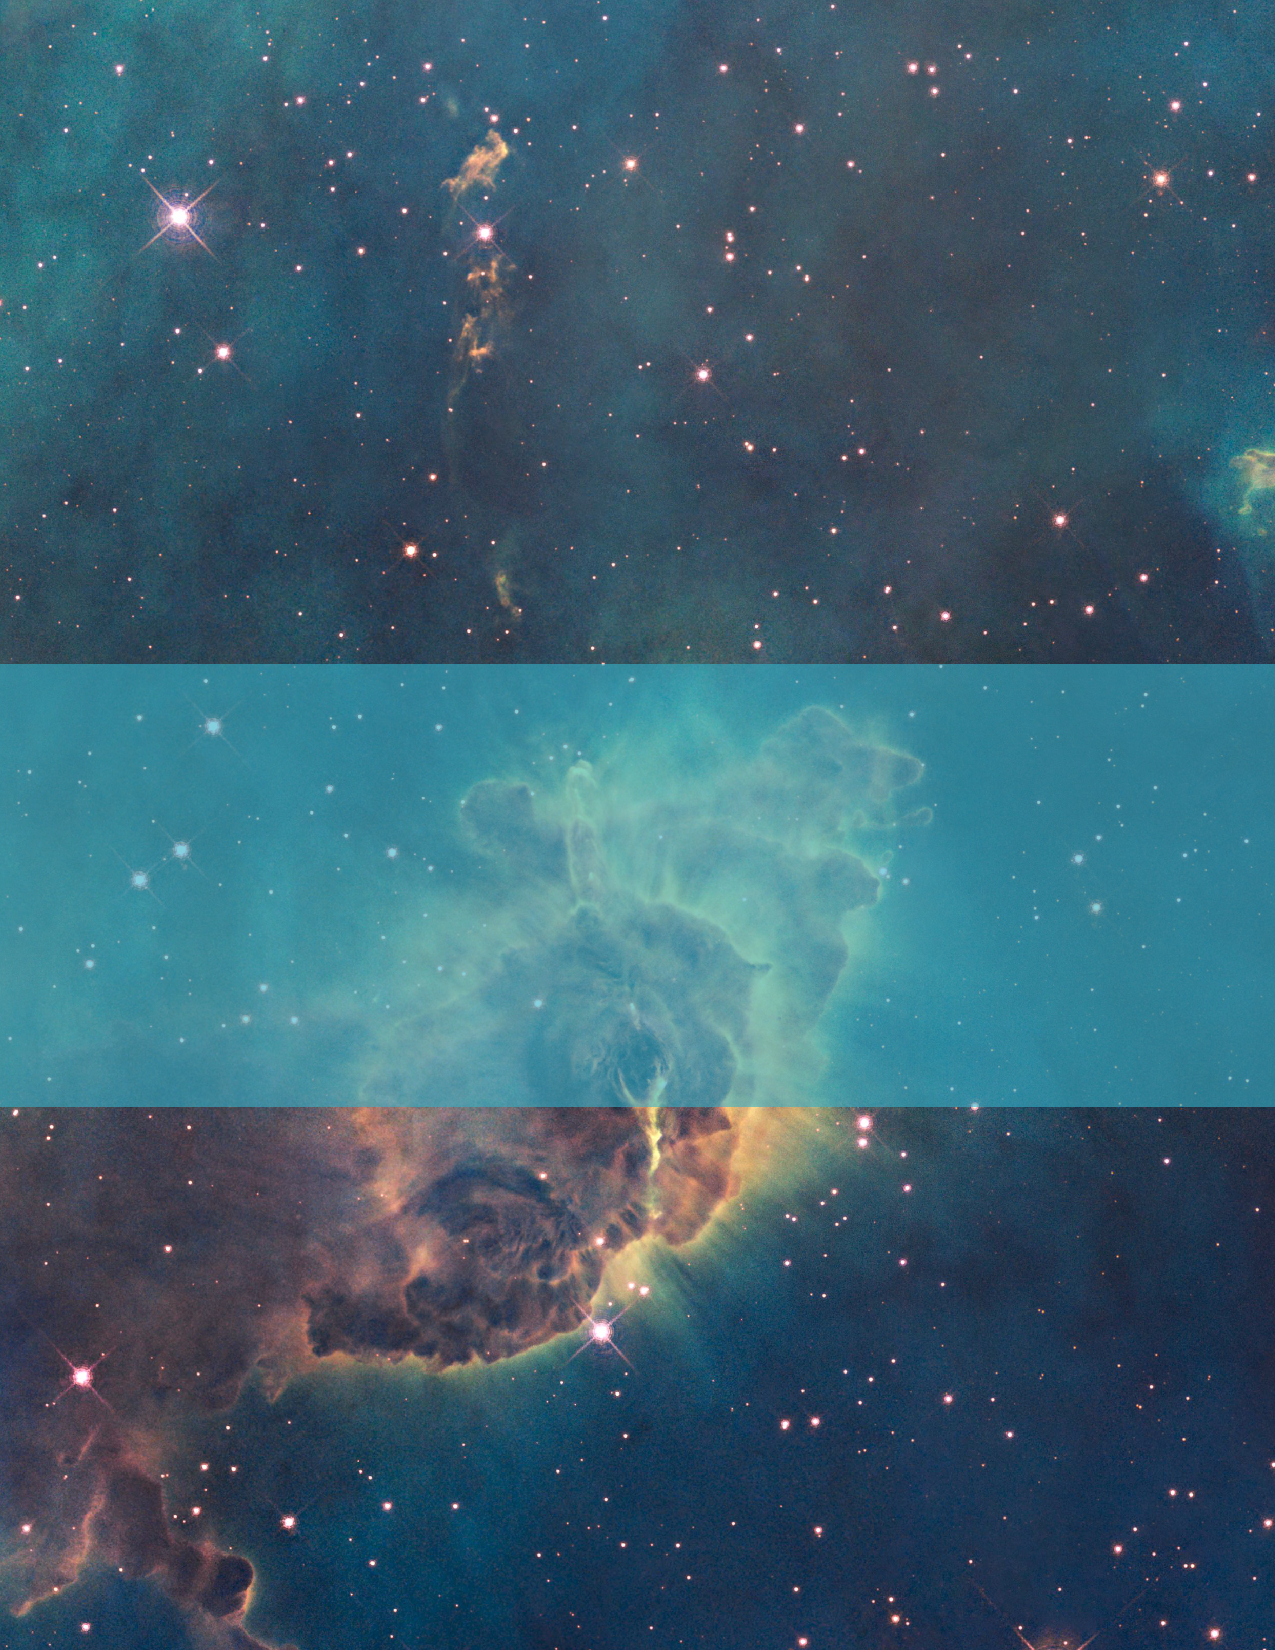
\includegraphics[scale=1.25]{esahubble}}} % Image background
\centering
\vspace*{5cm}
\par\normalfont\fontsize{35}{35}\sffamily\selectfont
\textbf{Astronomy notes}\\
{\LARGE Extragalactic Astrophysics}\par % Book title
\vspace*{1cm}
{\Large Shravya Shenoy}\par % Author name
\endgroup

%----------------------------------------------------------------------------------------
%	COPYRIGHT PAGE
%----------------------------------------------------------------------------------------

\newpage
~\vfill
\thispagestyle{empty}

%\noindent Copyright \copyright\ 2014 Andrea Hidalgo\\ % Copyright notice

\noindent \textsc{PhD Astronomy study notes}\\

%\noindent \textsc{github.com/LaurethTeX/Clustering}\\ % URL

\noindent This document is where I maintain my astronomy notes from different lectures and academic papers.\\ % License information

\noindent \textit{Last updated \today} % Printing/edition date

%----------------------------------------------------------------------------------------
%	TABLE OF CONTENTS
%----------------------------------------------------------------------------------------

\chapterimage{head1.png} % Table of contents heading image

\pagestyle{empty} % No headers

\tableofcontents % Print the table of contents itself

%\cleardoublepage % Forces the first chapter to start on an odd page so it's on the right

\pagestyle{fancy} % Print headers again

%----------------------------------------------------------------------------------------
%	CHAPTER 1
%----------------------------------------------------------------------------------------

%\chapter{Glossary}

This chapter contains a list of commonly used astronomy words and techniques, and their definitions.

\section{Source extraction}
Source extraction is a step in the process of astronomical image processing that calculates and reports the properties and characteristics of astronomical points of interest or sources. There are many software packages that automate the complex radio source identification and extraction process. Source Extractor is a very common tool to perform source extraction. Find a nice manual \textcolor{blue}{\href{http://star-www.dur.ac.uk/~pdraper/extractor/Guide2source_extractor.pdf}{here}}. Source Extractor is used for the automated detection and photometry of sources in fits imagefiles. SE works on scans of photographic plates as well as CCDs. 


\chapter{Introduction}
\section{Common equations}

\textbf{Stefan Boltzmann Equation}: related luminosity to temperature.
\begin{equation}
    L = 4 \pi R^2 \sigma_{SB} T^4
\end{equation}
where $\sigma_{SB}$ = 5.67 $\times$ 10$^{-8}$ W m$^{-1}$ K$^{-4}$.
The sun's effective temperature is 5780 K.

\section{Stellar spectra}
\begin{enumerate}
    \item The hottest stars are the bluest.
    \item Cool stars have absorption lines of neutral atoms or molecules and are usually redder.
    \item Balmer lines are relatively weak in O-type stars because hydrogen is almost fully ionized.
    \item A-type stars have the strongest Balmer lines because they are cool enough for hydrogen in the atmosphere to be largely neutral.
    \item \textit{\textbf{Are M-stars rich in Titanium?}} M-stars, cooler than 4000 K, show strong absorption bands of Titanium and Vanadium Oxide. It is NOT because M-type stars are rich in Titanium but because these molecules absorb red light very efficiently, and the atmosphere is cool enough for the molecules not to break apart. 
    \item Bands of TiO and VO are much weaker in L-type stars than M-type stars because most of the titanium and vanadium have condensed onto dust grains.
    
\end{enumerate}

\begin{figure}
    \centering
    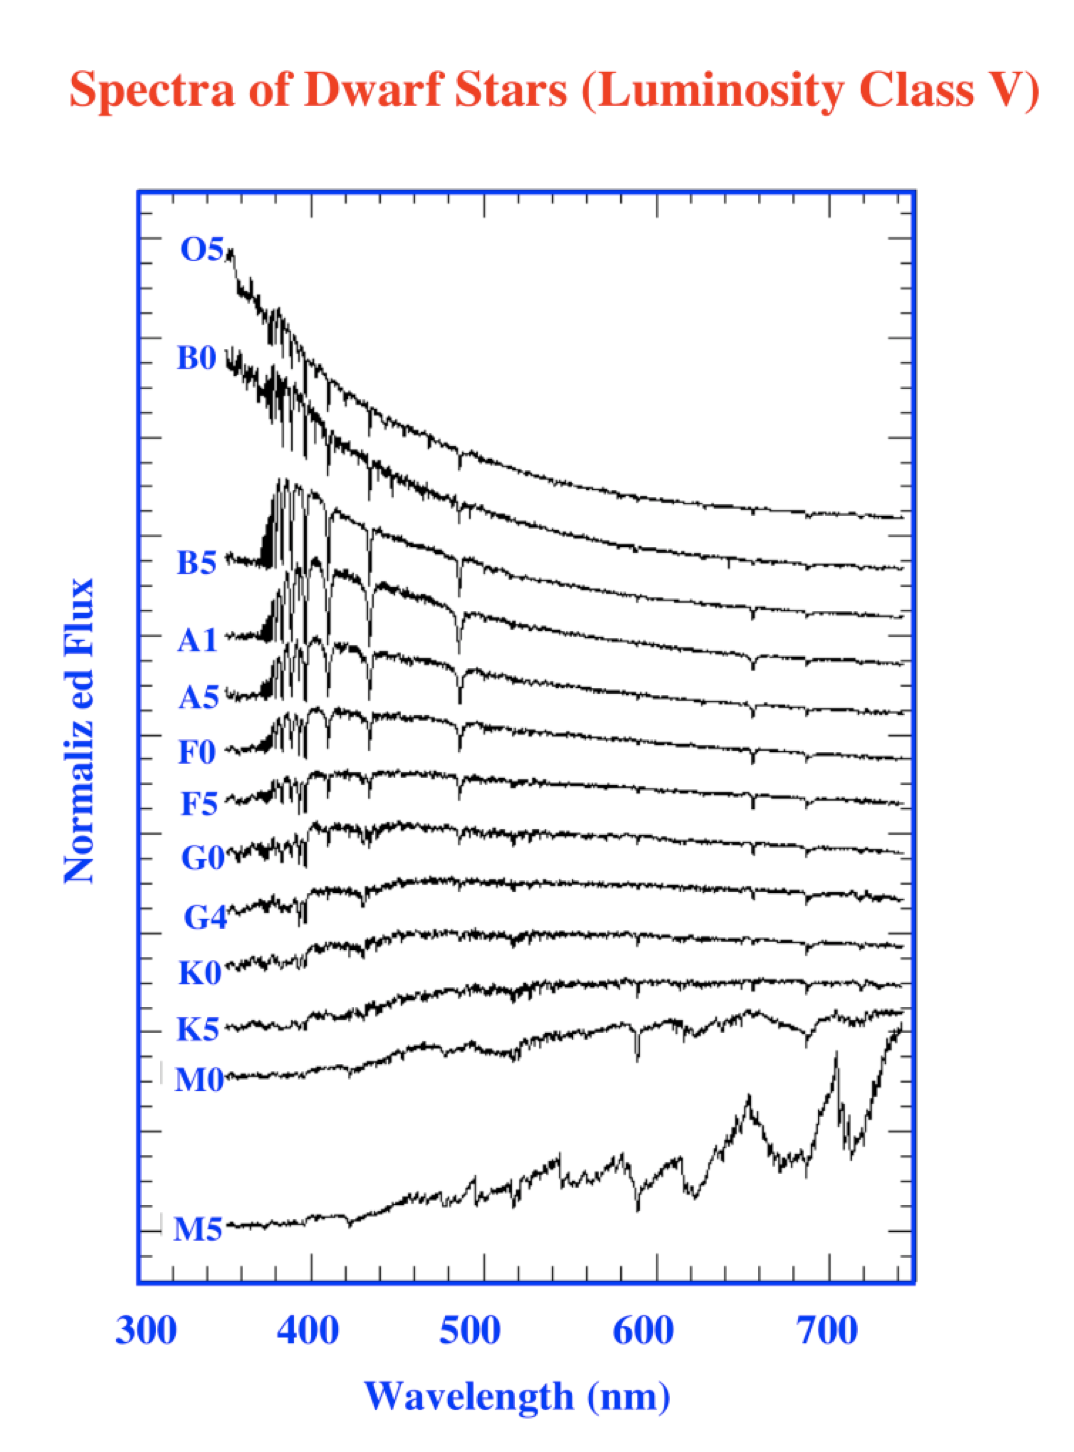
\includegraphics[scale=0.75]{Notes_Images/stellar_spectra.png}
    \caption{Stellar spectra from hottest to coldest. Notice how Balmer lines begin appearing only in A-type stars.}
    \label{fig:enter-label}
\end{figure}
\newpage
\begin{figure}
    \centering
    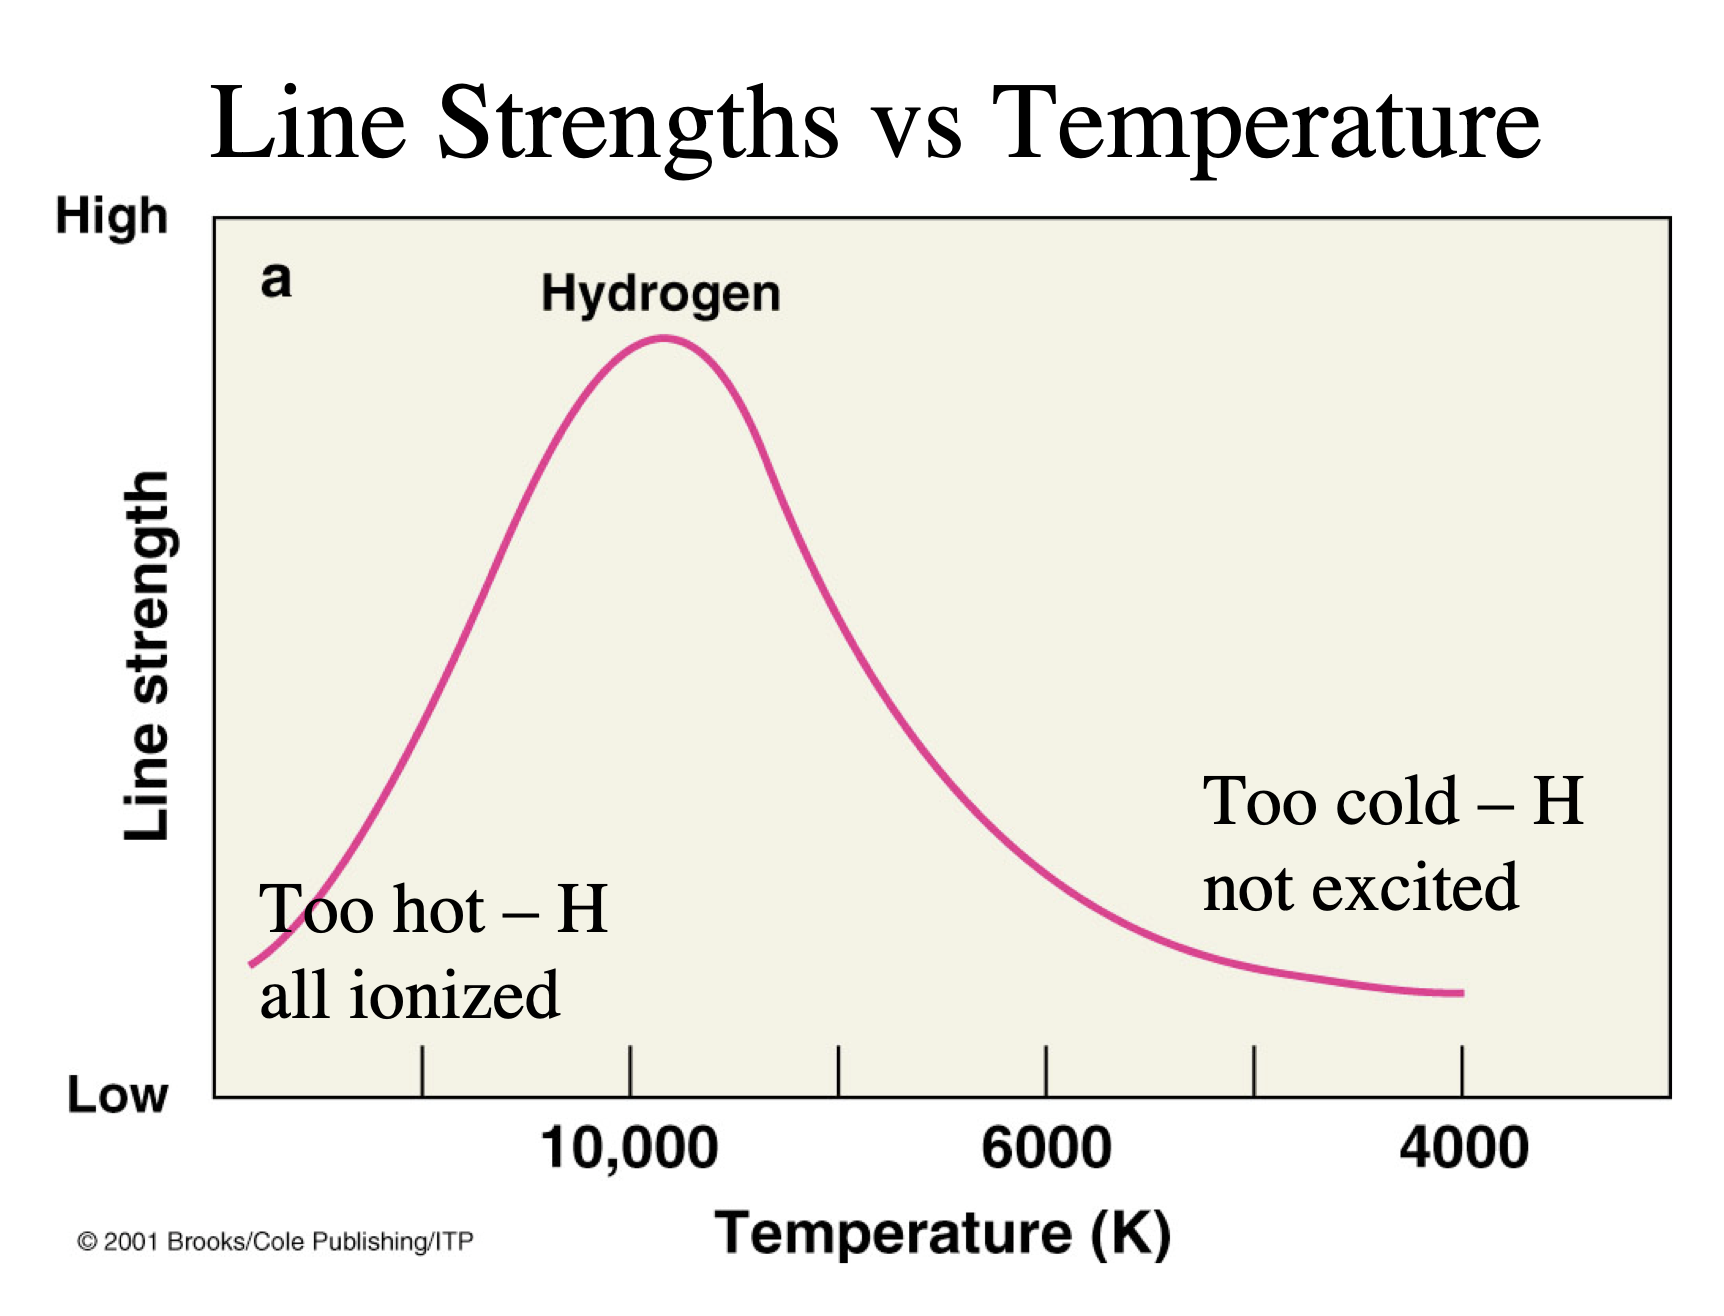
\includegraphics[scale=0.4]{Notes_Images/ionisation2.png}
    \caption{Caption}
    \label{fig:enter-label}
\end{figure}
\begin{figure}
    \centering
    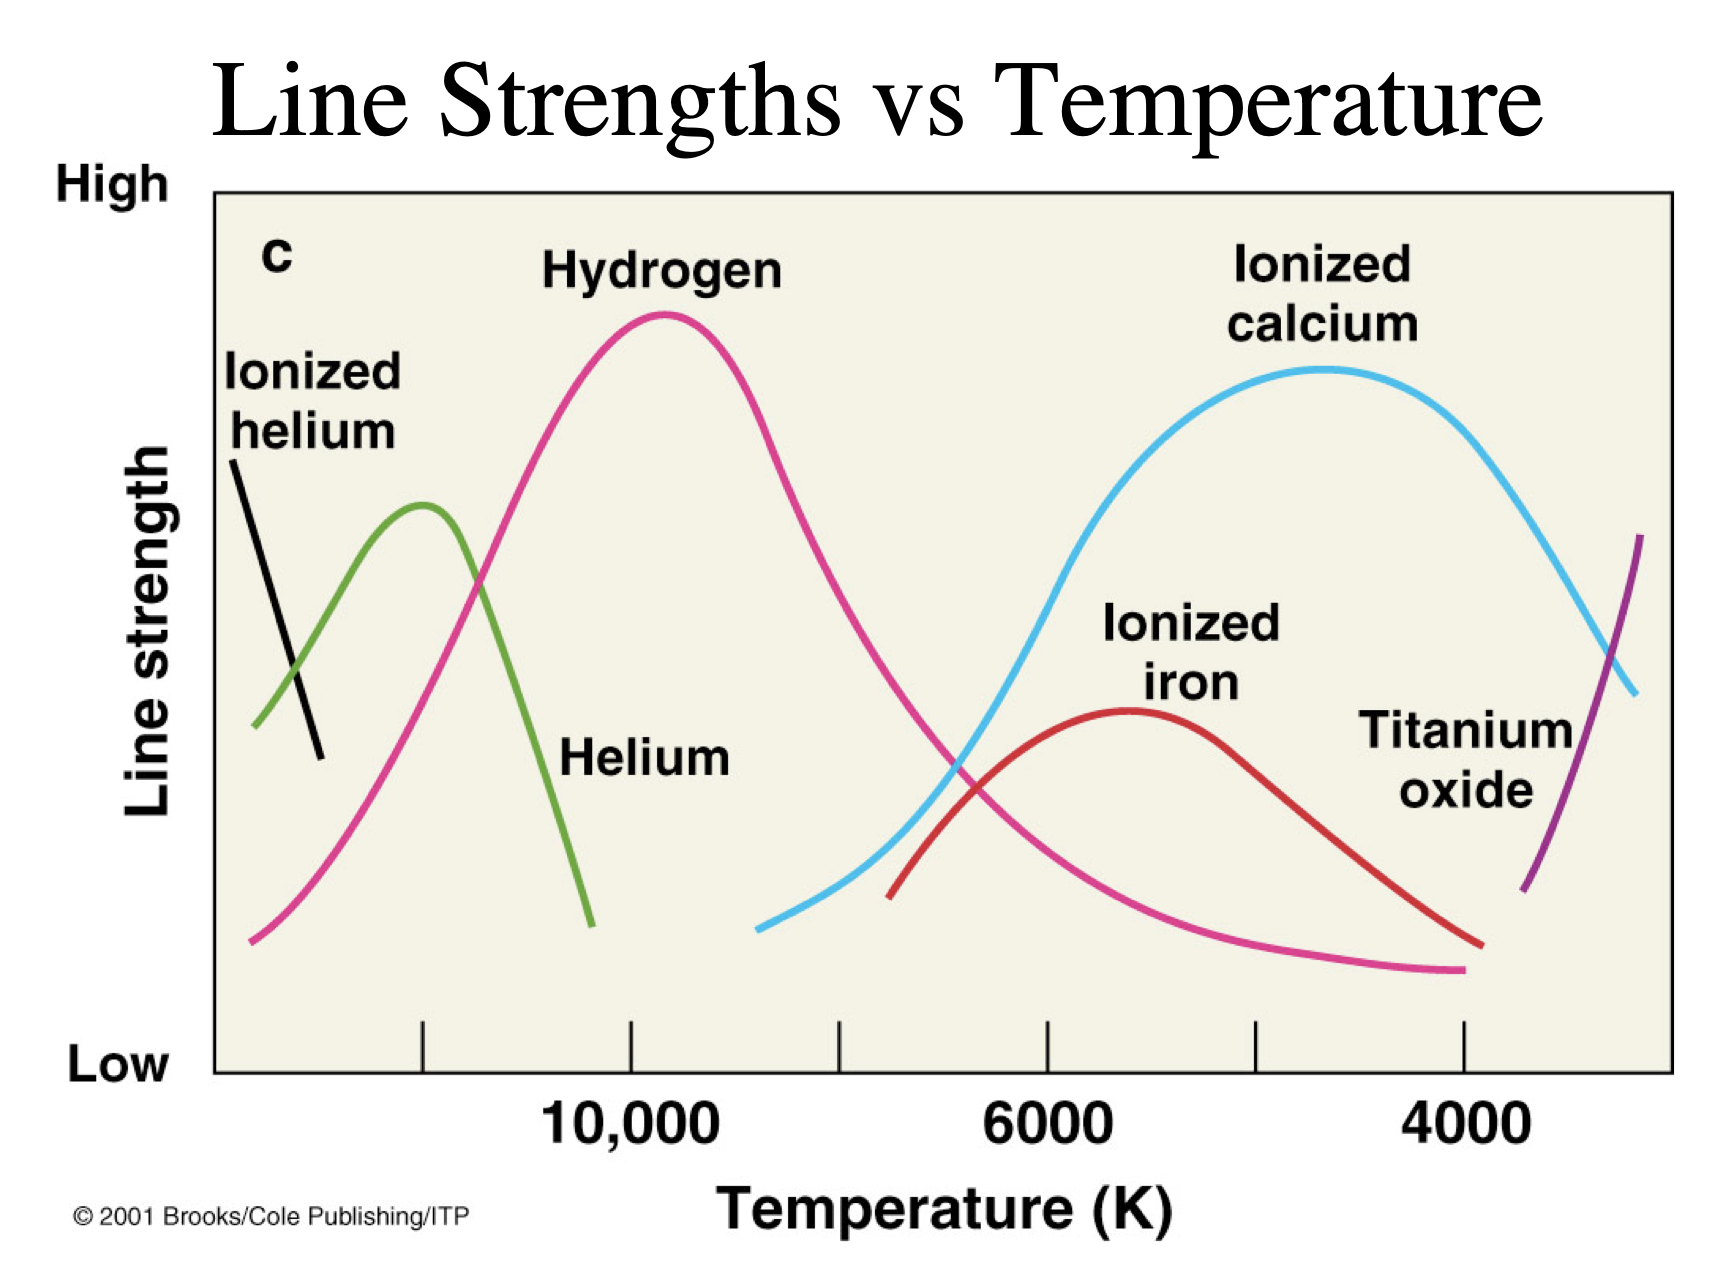
\includegraphics[scale=0.4]{Notes_Images/ionisation1.png}
    \caption{Caption}
    \label{fig:enter-label}
\end{figure}
\newpage
\chapter{AGN \& Quasars}

\section{Active Galactic Nuclei}

Active Galactic Nuclei (AGN  \footnote{Notes for this section taken from \href{https://www.isdc.unige.ch/~ricci/Website/Active_Galactic_Nuclei.html}{\textcolor{blue}{here}}} ) are the most luminous persistent sources of radiation in the Universe, and are powered by accretion onto a supermassive black hole (SMBH). In the last ten years it has become evident that most galaxies have gone through an AGN phase, which has played a crucial role in their formation and evolution. The typical AGN is made of several components (see Fig. \ref{fig:agn_schematic}):

\begin{enumerate}
    \item An accretion disk where matter is funneled onto the SMBH.
    \item A broad line region (BLR) where the broad and optical/UV lines are produced. Reverberation mapping studies have shown that the inner radius of this region scales with the luminosity and is  ~10-100 light days (e.g., Kaspi et al. 2005).
    \item A molecular torus, which is located within few parsecs from the SMBH. Near-IR reverberation studies have shown that the inner radius of the torus also scales with the luminosity (Suganuma et al. 2006).
    \item A narrow line region (NLR), which is located at ~100-300 pc from the SMBH, where the narrow optical lines are created.

\end{enumerate}

\section{Types of AGN }
Most AGN are radio-quiet, and can be divided into two classes \footnote{Kind of a misnomer- it doesn't mean there are two types of AGN, just means we have different viewing angles.}, according to their optical spectra. Type-I AGN, also called Seyfert 1s (Sy1s), show both broad and narrow lines, while type-II AGN (Seyfert 2s or Sy2s) show only narrow lines (see Fig. \ref{fig:seyfert_spectra}, taken from \href{https://reader.elsevier.com/reader/sd/pii/S1387647300000658?token=660DD777DEA7E41F7AD39364C79E4FA98C1E0C5C81431C48635052498601540CC37DC9AC7BA43B3AADF61AA5A59524EB&originRegion=eu-west-1&originCreation=20230127115455}{Pogge, 2000}). \\
\\
According to the simple unification model (e.g., Antonucci 1993), these objects are intrinsically the same, but are observed with different inclination angles with respect to the molecular torus (Fig. 3). \\
\colorbox{yellow}{Type-I are observed pole on, so that it is possible to observe both the BLR and the NLR, while} \\
\colorbox{yellow}{type-II are see edge-on, and the BLR is hidden by the torus.}

It is easier to discover a large number of Seyfert I in X-rays because 


Optical and soft X-ray surveys alone are highly biased toward only unobscured AGNs, while this simple WISE selection likely identifies even heavily obscured, Compton-thick AGNs.



\begin{figure}
    \centering
    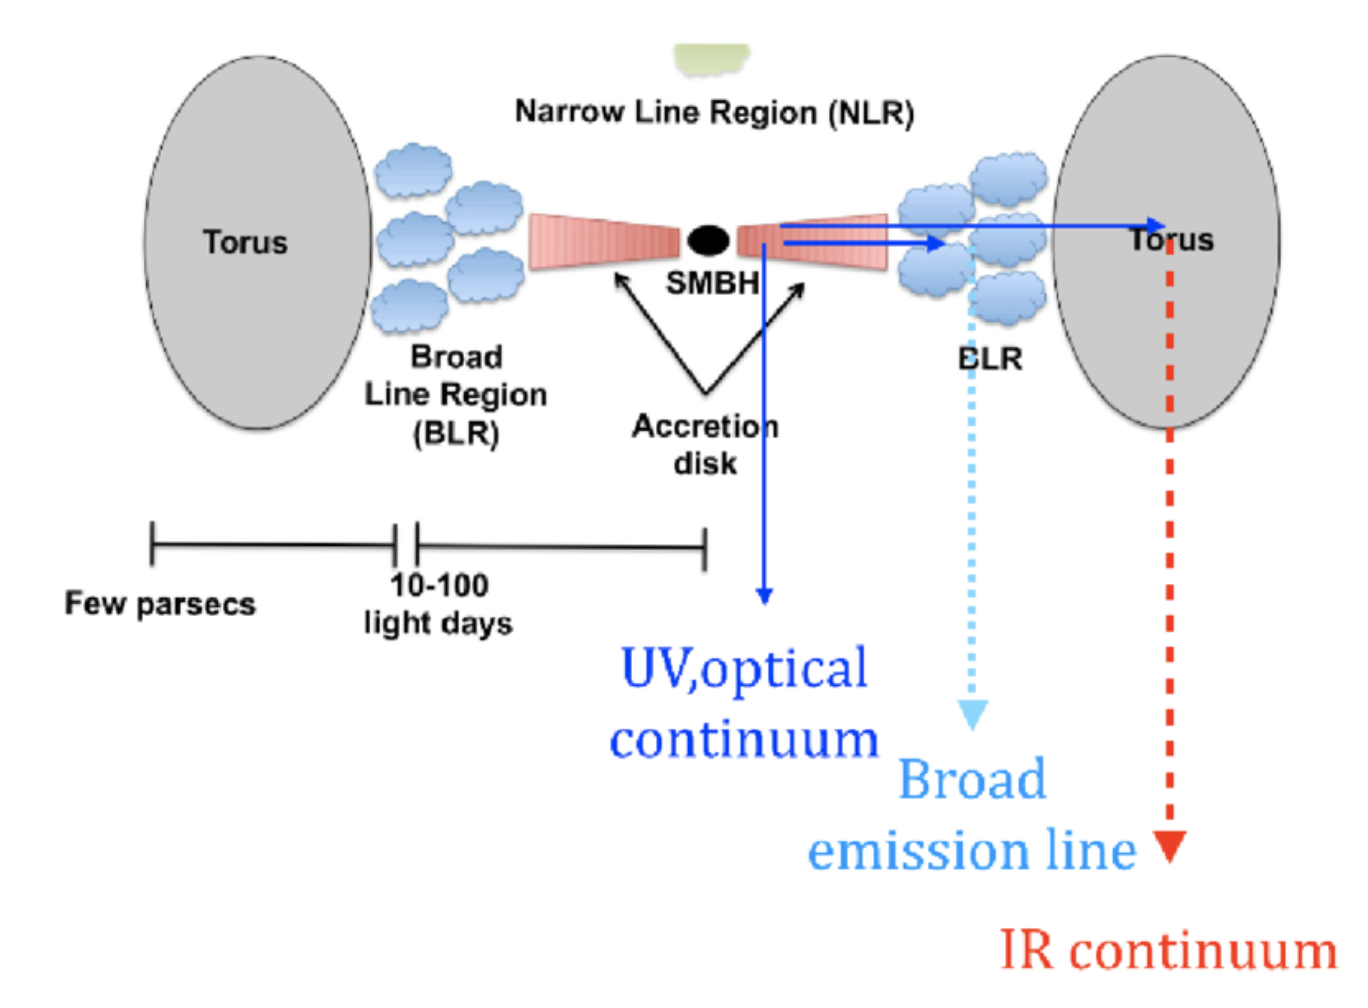
\includegraphics[scale=0.6]{Notes_Images/AGN_Schematic.png}
    \caption{Schematic diagram of the central structure of an AGN. Using the time lags among the light in different wavelengths, we will be able to estimate the physical size of each component (Image credit : Claudio Ricci)  }
    \label{fig:agn_schematic}
\end{figure}

\begin{figure}
    \centering
    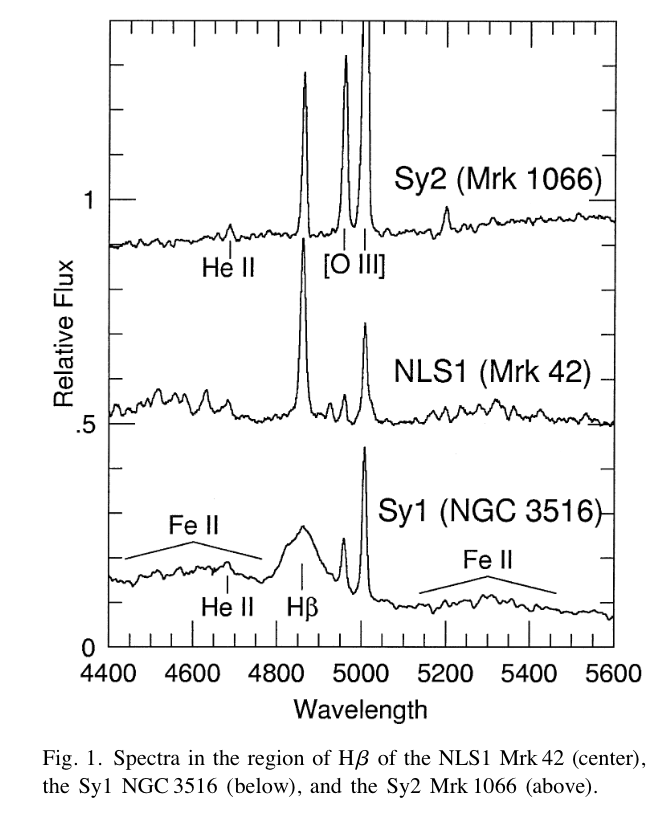
\includegraphics{Notes_Images/SeyfertsSpectra_Pogge.png}
    \caption{Spectra in the region of Hb of the NLS1 Mrk 42 (center),
the Sy1 NGC 3516 (below), and the Sy2 Mrk 1066 (above) taken from \href{https://reader.elsevier.com/reader/sd/pii/S1387647300000658?token=660DD777DEA7E41F7AD39364C79E4FA98C1E0C5C81431C48635052498601540CC37DC9AC7BA43B3AADF61AA5A59524EB&originRegion=eu-west-1&originCreation=20230127115455}{Pogge 2000}}
    \label{fig:seyfert_spectra}
\end{figure}

\section{Quasars}

\colorbox{yellow}{All quasars are AGNs, but not all AGNs are quasars.}\\
\\
 \href{https://arxiv.org/pdf/2007.12026.pdf}{Yesuf \& Ho 2020} : A recent far-infrared study indicates that \textbf{the gas content of the host galaxies of type 1 and type 2 quasars are similar}, and neither type is gas-deficient relative to normal, inactive galaxies (Shangguan \& Ho 2019). This is supported by the work of Zhuang \& Ho (2020), which is also based on the method of Yesuf \& Ho (2019).

\section{Hosts of AGN}
Griffith \& Stern 2010 find that the radio-selected AGNs are likely to be hosted by early-type galaxies, while X-ray- and mid-infrared-selected AGNs are more often associated with \textbf{point sources} and \textbf{disk galaxies}. 
%\include{Chapters/Asteroids.tex}
%\include{Chapters/Auroras.tex}
%\include{Chapters/BigBangTheory.tex}
\include{Chapters/Blackholes.tex}
%\chapter{Cold Gas}


\section{Gas and star-formation}
\href{https://www.annualreviews.org/doi/pdf/10.1146/annurev-astro-021022-043545}{\textcolor{blue}{Saintonge \& Cantinella 2022} :}From a gas perspective, there are three main factors that determine the star-formation rate of a galaxy, all three of which vary systematically across the local galaxy population: 
\begin{enumerate}
    \item the total mass of its cold ISM,
    \item how much of that gas is molecular,
    \item and the rate at which any molecular gas is converted into stars.
\end{enumerate}   

%\include{Chapters/Comets.tex}
%\chapter{Dwarf and Satellite galaxies}

\section{Dwarf Galaxies}

Dwarf galaxies are at the low end of SFR but reveal extended metal polluted haloes around them (Burchett et al. 2015; Bordoloi et al. 2014), which could be a sign of stellar feedback. 


\section{Satellite galaxies}

A satellite galaxy is a smaller companion galaxy that travels on bound orbits within the gravitational potential of a more massive and luminous host galaxy (also known as the primary galaxy). While \textbf{most satellite galaxies are dwarf galaxies} - not all, satellite galaxies of large galaxy clusters can be much more massive. The Milky Way is orbited by about fifty satellite galaxies, the largest of which is the Large Magellanic Cloud.\\
\\
\begin{enumerate}
    \item Satellite galaxies are identified in photometric catalogues using statistical background subtraction.
\end{enumerate}


\section{Ultra compact dawrf galaxies} \label{UCDs}

\cite{2008Mieske} state that a striking outcome of previous studies is the finding that the dynamical M/L ratios of massive compact stellar systems (UCDs) are, on average, about two times larger than those of normal glob- ular clusters of comparable metallicity.
\chapter{Extragalactic}

% -----------------------------
% -------- C G M --------------
% -----------------------------







\section{Circumgalactic Medium (CGM)}
\cite{2023VasilievEvgenii} : The discovery and intensive study of absorptions from heavy elements (such as CIV, SiIV, NV, OVI) in the circumgalactic medium (CGM) in quasar absorption spectra (e. g. Prochaska et al. 2006; Simcoe et al. 2006; Prochaska et al. 2017),  have posed \textbf{stellar feed-back} as one of the most important physical factors that determine, along with gravity, the structure and evolution of galaxies.


\section{Color-Color diagram}

A "colour" is the difference between two magnitudes, usually shorter minus longer wavelength, such that a positive colour means "redder". AGN can be identified using WISE colours. For example, Stern 2012 shows that the combined criteria W1 − W2 $\geq$ 0.8 and W2 $\leq$ 15 robustly identify an extremely robust, highly complete AGN sample. 

\begin{figure}
    \centering
    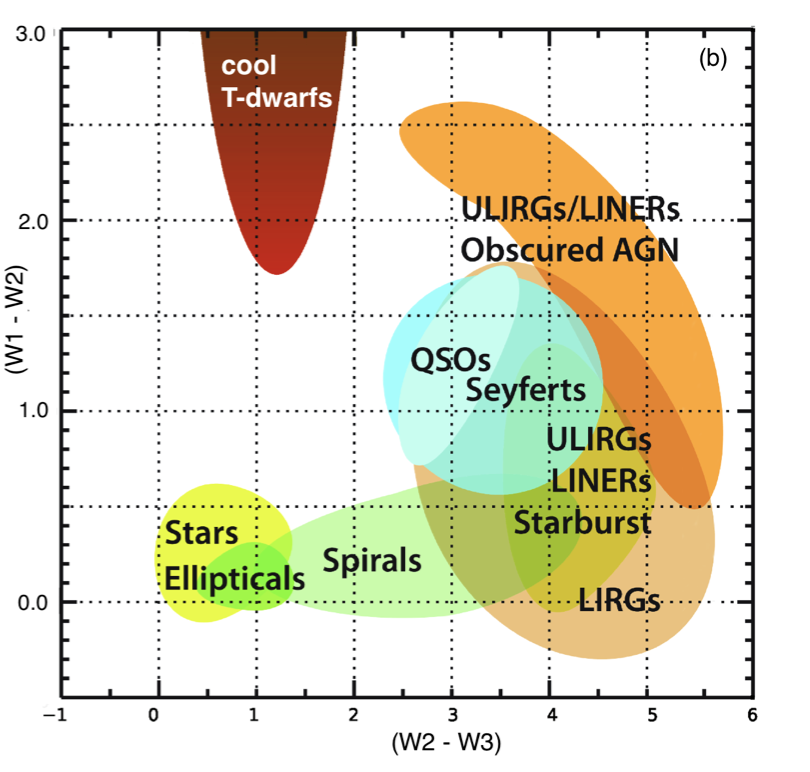
\includegraphics{Notes_Images/wise_color_color.png}
    \caption{W1, W2, and W3 stand for WISE magnitudes at 3.4, 4.6 and 12 $\mu$m, respectively. Based on the position of the galaxies on this plot, we can tell if they are star-forming spirals, cool stars or AGN. This plot is taken from Wright et al. 2010.  }
    \label{fig:enter-label}
\end{figure}


\section{Galactic Wind}

Galactic wind, a large-scale gas outflow from star formation in galactic discs, is thought to be driven by energy injection from young stars and supernovae in starburst events with a surface SFR exceeding a certain critical value. 
 The threshold for galactic winds driven by central starbursts is estimated at $ \varepsilon  \sim $ 10 erg cm $^{−2}$ s $^{−1}$ (Lehnert \& Heckman 1996a; Heckman 2000),  and for disc-halo circulation in edge-on galaxies $\varepsilon \sim$  10$^−3$ − 10$^−4$ erg cm$^{−2}$ s$^{−1}$ (Dahlem et al. 1995; Rossa et al. 2000; Dahlem et al. 2006). However, study of interrelations between the soft X-ray, UV, H$\alpha$, FIR and 1.4 GHz radio continuum emissions in a larger sample of 23 edge-on-galaxies led only to put a lower limit on the surface SN energy input rate $\varepsilon \geq$  10−3 erg cm$^{−2}$s$^{−1}$(Tüllmann et al. 2006).


\section{Galaxy Halos}

\cite{2023VasilievEvgenii} show that extended luminous haloes observed in edge-on galaxies (e.g., NGC891) can be maintained by disc-spread stellar clusters of smaller masses M$_∗$ $\sim < $  10 $^5$ M$_{\odot}$.



\section{Mid-infrared excess in galaxies}

Using a sample of $\sim$ 200 galaxies and active galactic nuclei (AGNs) from MOSDEF at 1.40< z< 2.61 with 24 $\mu$m detections (rest-frame 8 $\mu$m), \cite{2018Azadi} find that the Balmer line-derived SFRs or AGN activity are both not substantially higher in galaxies with mid-IR excess, alluding to the contribution of high mid-IR excess due to PAH contribution.




\chapter{Galaxies}

\section{Disc Galaxies}

\subsection{Barred Disc Galaxies}

Many disc galaxies host galactic bars, which exert time-dependent, non-axisymmetric forces that can alter the orbits of stars. \href{https://ui.adsabs.harvard.edu/abs/2023arXiv230201307F/abstract}{\textcolor{blue}{Filion+2023}}  find that the \textbf{bar induces both azimuth angle- and radius-dependent trends} in the median distance that stars have travelled to enter a given annulus. Angle-dependent trends are present at all radii they considered, and the \textbf{radius-dependent trends roughly divide the disc into three ‘zones’.} In the inner zone, stars generally originated
at larger radii and their orbits evolved inwards. Stars in the outer zone likely originated at smaller radii and their orbits evolved outwards. In the intermediate zone, there is no net inwards or outwards evolution of orbits. They comment on the possibility of using observed angle-dependent metallicity trends to learn about the initial metallicity gradient(s) and the radial re-arrangement that occurred in the disc.


\section{Stellar Mass}


\section{Stellar mass and velocity dipersion}
\href{https://iopscience.iop.org/article/10.3847/0004-637X/832/2/203/pdf}{Zahid+2016} :The stellar mass and velocity dispersion are governed by different physical processes, but both are intimately related to properties of the dark matter halo. \textbf{Stellar mass and velocity dispersion are strongly correlated, making it difficult to determine which of these two parameters is fundamental}. The stellar mass is an integral over the star formation history (SFH) and the end product of the complex baryonic processes governing galaxy formation and evolution. In contrast, the velocity dispersion is a measure of the stellar kinematics and is directly related to the gravitational potential of the system.



\section{Velocity Dispersion}

For spiral galaxies, the increase in velocity dispersion in population I stars is a gradual process which likely results from the random momentum exchanges, known as \textbf{dynamical friction}, between individual stars and large interstellar media (gas and dust clouds) with masses greater than 10$^5$ M$\odot$. Face-on spiral galaxies have a central $\sigma$ $\leq$ 90 km/s; slightly more if viewed edge-on.
\\

\textbf{Determining mass using H alpha}: The H-alpha line saturates (self-absorbs) relatively easily because hydrogen is the primary component of nebulae, so while it can indicate the shape and extent of the cloud, it cannot be used to accurately determine the cloud's mass. Instead, molecules such as carbon dioxide, carbon monoxide, formaldehyde, ammonia, or acetonitrile are typically used to determine the mass of a cloud.



\chapter{Globular Clusters}

\section{Globular Clusters vs Satellite galaxies}

Both globular clusters, as well as satellite galaxies, can be found in the halo of a primary galaxy. However, they are different. Satellite galaxies are not only more extended and diffuse compared to globular clusters but are also enshrouded in massive dark matter halos that are thought to have been endowed to them during the formation process. 

\section{Globular Clusters}

Formation of globular clusters may have a link with the formation of \textbf{ultra-compact dwarf galaxies (UCDs;} see \ref{UCDs}), star cluster size systems with mass in the range of 10$^6$ solar mass - 10$^8$ solar mass and half mass radii of 10-100 pc. 


%\chapter{Gravitational Lensing}


\section{What is gravitational lensing?}

\textbf{How do you estimate accurate redshift of a lensed galaxy?}
Does spectra shift when a galaxy is gravitationally lensed?
\\
\\
\href{https://ui.adsabs.harvard.edu/abs/2023arXiv230111264M/abstract}{Mainali et al. 2023} -- present new observations of sixteen bright (r = 19 − 21) gravitationally lensed galaxies at z $\simeq$ 1−3 selected from the CASSOWARY survey. In this paper, they investigate the rest-frame UV nebular line emission in our sample with the goal of understanding the factors that regulate strong CIII] emission. They compare the rest-optical line properties of high redshift galaxies with strong and weak CIII] emission, and find that systems with the strongest UV line emission tend to have young stellar populations and nebular gas that is moderately metal-poor and highly ionized, consistent with trends seen at low and high redshift. They find that \colorbox{yellow}{gas traced by the CIII] doublet likely probes higher densities than that traced by [OII] and [SII].} \\ Characterisation of the spectrally resolved Mg II emission line and several low ionization absorption lines suggests neutral gas around the young stars is likely optically thin, potentially facilitating the escape of ionizing radiation.


\section{Influence of lensing on the spectra : QSOs}

Recently Wandel, Peterson \& Malkan (1999) and Kaspi et al. (2000) using the reverberation technique discovered that the size of the \colorbox{yellow}{broad-line region (BLR; see Fig. \ref{fig:agn_schematic}) was smaller than that assumed} in the standard active galactic nucleus (AGN) model.

\chapter{Galaxy Mergers }


\section{Formation of bars}

There are three models of bar-formation considered in \href{https://arxiv.org/pdf/2006.14847.pdf}{Cavanagh et al. 2020}:
\begin{enumerate}
    \item Isolated model : Holh 1971 found that slow-growing non-axisymmetric disturbances eventually led to the formation of a central bar structure.
    \item Tidal model
    \item Merger model
\end{enumerate}

Mergers with \textbf{low mass ratios} and closely-aligned orientations are \textbf{more conducive} to bar formation than equal-mass mergers (\href{https://arxiv.org/pdf/2006.14847.pdf}{Cavanagh et al. 2020})

\section{Presence of bars in spirals}

"Around 30\% of all spiral galaxies are understood to be strongly barred (Sellwood \& Wilkinson 1993), while overall, more than 50\% of spiral galaxies typically contain features indicative of a central bar structure (Eskridge \& Frogel 1999). Bars are found to be even more prevalent when observed in infrared (Eskridge et al. 2000)." (\href{https://arxiv.org/pdf/2006.14847.pdf}{Cavanagh et al. 2020})
%\include{Chapters/Planets.tex}
\chapter{Stars and Supernovae}



\section{Supernovae}


\subsection{Types of supernovae\footnote{Text for Sec. \ref{SNTypes} and Fig. \ref{fig:supernova} are taken from 
 \href{https://astronomy.com/magazine/2004/08/know-your-supernovae}{here}.}} \label{SNTypes}

\begin{figure}[!h]
    \centering
    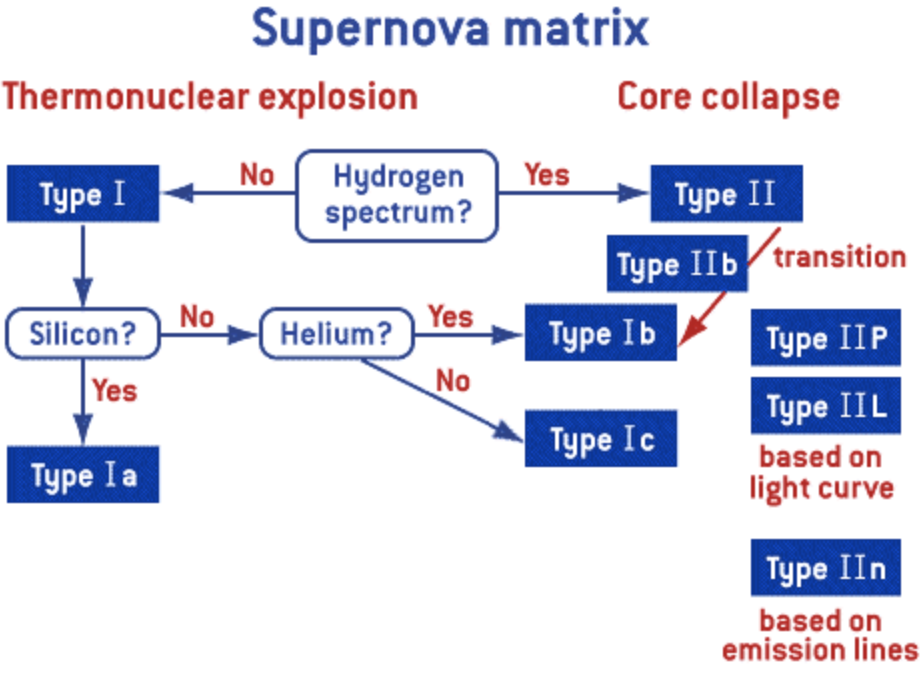
\includegraphics[scale=0.6]{Notes_Images/Supernovae.png}
    \caption{We distinguish supernova types mainly on the basis of their spectra. This illustration relates observed characteristics to the mechanism thought responsible for the explosion.}
    \label{fig:supernova}
\end{figure}

\subsubsection{Type Ia Supernova}

These usually occur in binary systems (two stars orbiting one another) in which one of the stars is a white dwarf. The Type Ia category of supernova produces a fairly consistent peak luminosity because of the fixed critical mass at which a white dwarf will explode - also called Chandrasekar Limit of 1.44 $M_{\odot}$. \textbf{Example}: SN 2001el in NGC 1448

\subsubsection{Types Ib and Ic}

These supernovae types represent the collapse of a massive star. No hydrogen or silicon lines are present in the spectrum, but type Ib spectra show helium. Found only in spiral galaxies, type Ib and Ic supernovae are thought to be associated with massive stars that have lost their hydrogen envelopes either by strong stellar winds (as in Wolf-Rayet stars) or mass loss to a binary companion. Light from these supernovae tends to be more highly polarized, implying more asymmetric explosions among this class. \textbf{Examples: }SN 1998bw (GRB 980425) and SN 2003dh (GRB 030329)

\subsubsection{Type II }

Prominent hydrogen lines are seen in this supernova type's spectrum. These events are associated with regions of recent star formation. They are not found in elliptical or early-type spiral galaxies. This class often is subdivided as IIP (plateau) and IIL (linear) based on how the optical brightness declines. Type IIL supernovae originate from stars retaining much smaller hydrogen envelopes (approximately 1 to 2 solar masses) than progenitors of IIP (typically 10 solar masses) supernovae. \textbf{Example:} SN 1987a in the Large Magellanic Cloud

\subsubsection{Type IIn}

A strong hydrogen spectrum is present with narrow emission lines for this type of supernova. IIn supernovae are thought to originate from the collapse of massive stars embedded in dense shells of material ejected in the decades leading up to the explosion. \textbf{Example}: SN 1998s in NGC 3877

\subsubsection{Type IIb}

The spectrum of this type of supernova contains prominent hydrogen lines right after the event but later transitions to something resembling a Type Ib/c supernova. The progenitor is thought to be a red supergiant that has lost most of its hydrogen envelope either through strong stellar winds or through mass loss to a nearby companion star. IIb supernovae are seen as a "missing link" between supernovae that have retained their envelopes and those that have not. \textbf{Example:} SN 1993j in M81



\section{AGB stars}

Asymptotic Giant Branch (AGB) stars are evolved, low- to intermediate-mass stars ($\sim$ 0.8 − 8M$\odot$) that are characterised by significant mass loss due to a dust-driven wind (Bowen 1988, \href{https://arxiv.org/pdf/2304.05924.pdf}{S. Maes et al. 2023}) As a result, this outflow creates a vast circumstellar envelope (CSE).\\
\\
The type of chemistry in the CSE is set by the elemental carbon-to-oxygen (C/O) ratio of the AGB star, with C/O < 1 resulting in oxygen-rich outflows and C/O > 1 resulting in carbon-rich outflows. AGB outflows with C/O $\sim$ 1 are called \textbf{S-type AGB}. \\
\\
\textbf{Outflow Chemistry:} 
In O-rich AGB outflows, the chemistry is dominated by reactions with the parent species H2O and its daughter OH. Chemistry in C-rich outflows is more diverse since carbon is very reactive, readily producing many carbon-based molecules and ions. 
\chapter{Star formation in galaxies}

\section{Regulation of SF}

Processes like magnetic fields and turbulence regulate the star forming efficiency by acting against this collapse. But the most important mechanism that regulates collapse is self-regulation (Yan et al. 2023): when stars form in MCs, protostellar winds and massive OB stars destroy the clouds via ionization, heating by ultraviolet photons, stellar winds, and supernova blast waves. Although these processes can quench star formation locally, the shock waves can compress gas in another cloud, inducing star formation globally. These processes play an important role that regulates galaxy
formation and evolution.


For star formation to take place, gas and dust need to be sufficiently cold for gravity to overcome thermal pressure, and the ionisation fraction must be low enough to enable substantial decoupling between the gas and the Galactic magnetic field.



\href{https://arxiv.org/pdf/2303.05054.pdf}{This paper} used a spatially resolved SED to observe modestly suppressed star formation in the inner kiloparsec of the galaxy, which suggests that we are witnessing the early stages of inside-out quenching. They develop a parametric lens model to reconstruct the source-plane structure of dust imaged by the Atacama Large Millimeter/submillimeter Array, far-UV to optical light from Hubble, and near-IR imaging with 8 filters of JWST/NIRCam, as part of the Prime Extragalactic Areas for Reionization and Lensing Science (PEARLS) program.
%\chapter{Spectroscopy}

 Among ion–ion correlations, \cite{Burchett_2015} find evidence for tight correlations between C II and Si II, C II and Si III, and C IV and Si IV, suggesting that these pairs of species arise in similar ionization conditions. However, the evidence for correlations decreases as the difference in ionization potential increases. When controlling for observational bias, they find only marginal evidence for a correlation (86.8\% likelihood) between the Doppler line width b(C IV) and column density N(C IV).


\section{Fitting emission lines}

One assumption people make while fitting emission lines is that the detected lines can be fitted simultaneously under assumption of local thermodynamic equilibrium (LTE). 

 Second, the effects of dielectronic recombination may contribute to enhancing the level populations even at large n.

 \section{Radio recombination lines}

 

 Radio recombination lines (RRLs) are commonly defined as radio spectral lines resulting from \textbf{transitions of high-n levels} of atoms, appearing after the \textbf{recombination of singly inoized ions and electrons} \href{https://ui.adsabs.harvard.edu/abs/2002ASSL..282.....G/abstract}{\textcolor{blue}{(Gordon \& Sorochenko 2002)}}\\
 \\
 \subsubsection{RRLs of ions with mass higher than Helium}
Searching for RRLs of ions heavier than helium towards the Sun has been unsuccessful (Berger \& Simon 1972); \href{https://link.springer.com/article/10.1134/S1063772922060038}{\textcolor{blue}{(Dravskikh \& Dravskikh 2022)}}.\\
\\
 \href{https://arxiv.org/pdf/2302.03398.pdf}{\textcolor{blue}{Liu Xunchuan+2023}} report the first detection of radio recombination lines (RRLs) of ions heavier than helium. In a highly sensitive multi-band (12–50 GHz) line survey toward Orion KL with the TianMa 65-m Radio Telescope (TMRT). 
%\chapter{Surveys}

%\include{Chapters/Telescopes.tex}



\addcontentsline{toc}{chapter}{\textbf{Bibliography}} 
\begingroup
\renewcommand\thechapter{}
\titleformat{\chapter}[display]
{\normalfont\huge\bfseries}{}{20pt}{\Huge}
\bibliographystyle{aasjournal}
\bibliographystyle{aasjournal}
\bibliography{refs}
\endgroup

\end{document}